\chapter{Preliminary Results}
\julian{I'm unsure how best to describe and structure my findings. For now, this chapter will be the focal area that include information provided by others e.g. their observations and perceptions and - eventually - the results of actually applying these concepts for real apps}.

% The following was removed from the Introduction, some of it may be used at the end of the thesis. 
\section{My contributions in this thesis}\label{my-contributions-in-this-thesis}
I have introduced the concept of using mobile analytics to help illuminate emergent behaviours of mobile apps and set mobile analytics into a broader context of other sources and reflections of perceived quality of mobile apps.

I have contributed the first studies into Platform Analytics as provided by Google Play Console, including pre-launch reports and Android Vitals, services intended to help developers identify quality issues with their Android apps in order to address these issues so they do not affect end-users. I have helped demonstrate their efficacy, despite various flaws I also discovered, identified and reported to Google. 

\begin{figure}[ht]
    \centering
    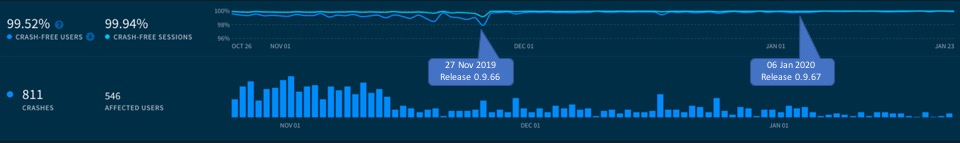
\includegraphics[width=\textwidth]{images/annotated_pocketcode_90_day_fabric_crashlytics_report.jpg}
    \caption{Pocket Code improvements in crash rate, in 90 days}
    %\Description{Pocket Code: When the project team investigated crashes they improved the reliability}
    \label{fig:pocketcode_improvements_in_crash_rate}
\end{figure}

Through my work with the key app created by the Catrobat project team we tamed their key Android app's crash rate that was previously precariously high\footnote{Nearly four times the maximum threshold recommended by Google in their Android Vitals service.}. The project team had not been able to address the crash rate despite applying many of the recognised and recommended software development practices over several years~\cite{adamsen2015systematic_catrobat, luhana2018streamlining, ali2019behavior_catrobat, ali2019using_catrobat, hirsch2019approach_catrobat, schranz2019contributors_catrobat, slany2014tinkering}. Owing to my involvement we were able to achieve this within 90 days and 2 releases through several small improvements to the codebase of the app, as Figure \ref{fig:pocketcode_improvements_in_crash_rate} shows.

\akb{I think you need to emphasise the role of analytics over your personal role above}

I also compare Crashlytics reports with the Platform Analytics and again identify both internal and cross-tool flaws and inconsistencies. Some of these have already been reported to Google in preparation for a full report to be submitted on completion of some ongoing research.

\begin{figure}[ht]
    \centering
    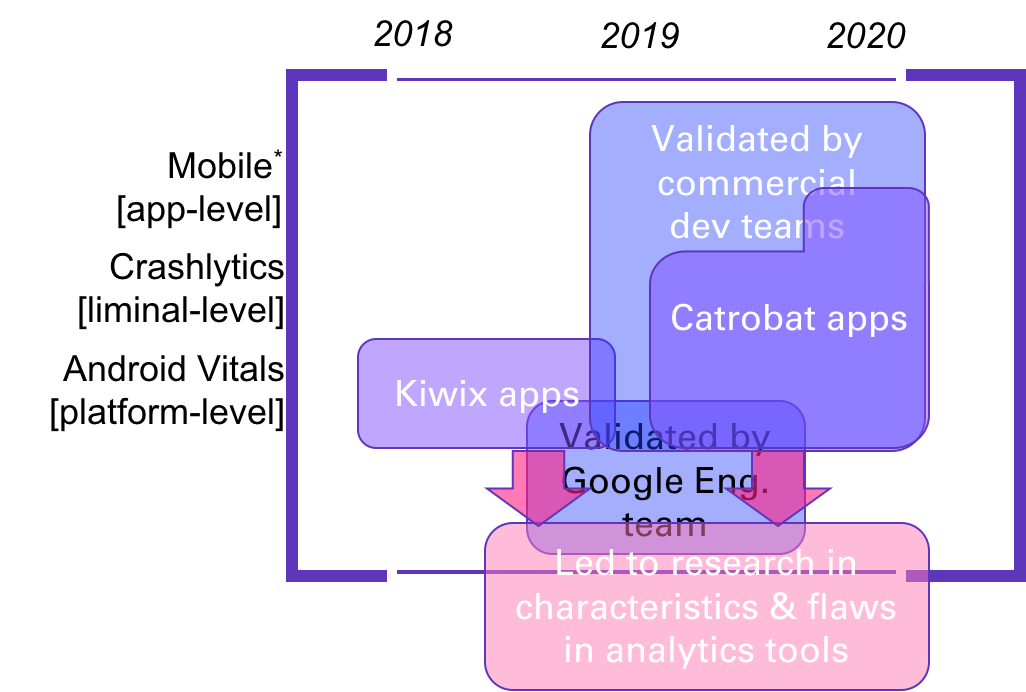
\includegraphics[width=10cm]{images/visual-connections-in-research.png}
    \caption{Visual Connections in my research}
    \label{fig:visual-connections-in-research}
\end{figure}

Figure \ref{fig:visual-connections-in-research}  aims to provide a visual overlay of the main practical elements of the research from 2018 to 2020. There are three main factors: 1) the type(s) of analytics used, 2) the development team and their apps, and 3) timescales.
\akb{Why is it important to understand the timeline here - what implication does it have for understanding the research problem?}

The research started with the Kiwix~\footnote{The Kiwix project enables people to use Wikipedia and other content offline~\url{https://www.kiwix.org/en/}} set of Android apps where the app with the highest crash rate, as reported by Google's Android Vitals, was used as the experiment to see if the crash rate could be improved. By design the Kiwix apps do not include any analytics or crash reporting to minimise the digital usage footprint of these apps as they may be used in areas of the world where Wikipedia is banned, \emph{etc.} where the users may be persecuted or even imprisoned. Nonetheless, as the apps were available through Google Play (amongst many sources) the development team received ongoing reports in Google Play Console including the Android Vitals reports on various `stability' metrics as defined and applied by Google. 

Google Play uses data collected automatically from users opted-in to provide usage and diagnostics data to Google. The data is collected at a per-device level, which means that one device could potentially report data from several user accounts, conversely for users who use multiple devices some may provide the data while others do not.

The Catrobat team was and is an extremely well researched and supported collection of mobile apps intended to help young people learn how to enjoy developing games visually. It was established by Professor Wolfgang Slany of the TU Graz university where both undergraduate and postgraduate students actively practice software skills on the codebase. My engagement started around June 2019 and we jointly decided to pick the thornier and most complex Android app - Pocket Code - as the subject for our collaboration and research as it had proved to have an intractable ongoing issue with the high reported crash rate and therefore a worthy challenge for the concepts proposed in my research. We had a reference app, called Pocket Paint, which had a lower crash rate. Note: Pocket Paint was and is incorporated into Pocket Code in addition to being a standalone app.

Pocket Code already incorporated one of the most popular crash analytics library called Crashlytics. At the time, it used an older, mature version of Crashlytics branded Fabric (a business first acquired by Twitter, then by Google). I have chosen to use the term \emph{liminal}~\footnote{\url{https://www.lexico.com/en/definition/liminal}} to indicate crash reporting is something that lives in the boundary layer between the app and the operating system, or platform. Either is able to observe application crashes, and for apps where both the app and the platform capture information about crashes the two data sources can be usefully cross-referenced and compared, as my research has done.

As Pocket Code was an Android app, available in Google Play, the team also received the reports provided by Google through Google Play. These two data sources provided an interesting and rich set of research challenges. 

Relatively recently, in February 2020, the Catrobat team had to migrate their Crashlytics reporting from the Fabric service, which Google was ceasing, to Firebase the replacement reporting service Google provided. In parallel with this migration of the reporting the project team agreed to incorporate mobile analytics into their Android and iOS apps. They decided to use Firebase Analytics for various reasons (to be covered later in my thesis), hence the extension of the apps into app-level analytics.

The two arrows in the figure indicate an area of unplanned research: 
%
I discovered various flaws in the developer-oriented reports Google provides to app developers who make their apps available in Google Play (approximately 2.9 million apps globally). This led initially to discussions with the relevant engineering teams for Google Play and Android Vitals at Google where they confirmed various flaws. They asked for ongoing updates on my findings and requested a report which I provided. Through our interactions and discussions I realised the merit of researching the characteristics and flaws in analytics tools, and particularly those provided by Google for Android developers. This research is ongoing and intended to continue post PhD given the importance and relevance of the topic.

In mid-2019 several commercial Android development teams learned of my research and offered to contribute their experiences and practices of using mobile analytics in their commercial apps. These apps include app-level analytics in addition to the development teams receiving the ongoing reports Google provides automatically. The contributions of these development teams helped provide additional weight to the value and relevance of using mobile analytics to identify flaws in mobile apps and evidence of the importance developers placed on addressing quality issues gleaned through these tools.

%\yy{The practical research}{Need to complete the sentences, what is liminal? Change Kiwix/Catrobat apps to "Kiwix/Catrobat teams"? }

I instigated and led the development of several opensource software utilities to help record and preserve reports and underlying failure data from Google Play Console and Android Vitals. We have successfully extended the capabilities of the utilities and further extensions are practical. Research benefits:
\begin{itemize}
    \item Evidence preserved for analysis:
    \item Data can now be compared and further assessed:
    \item Data and contents can be shared by developers of Android apps with other researchers - extending the body of knowledge about crashes (un-reliability) and ANRs (run-time unresponsiveness). \emph{bringing previously unknown data, practices and tools into the open so others can understand them, make more informed decisions, and perform further research.}
\end{itemize}

I made data available~\cite{harty_wama_dataset_examples} for further research based on data originally only made available to app developers. Larger volumes of data are available upon request.

The research has been presented at various conferences and workshops, including at NII Shonan in 2019 at meeting 152 on "Release Engineering for Mobile Applications"~\footnote{~\url{https://shonan.nii.ac.jp/seminars/152/}}. 
